To build and install microML on a *\textit{Nix} system there is an installation script in the main directory
of the repository. This does not need to be run with sudo permission. See
Appendix~\ref{appendix:samples}.  To build and install microML ensure that
\textbf{stack}\footnote{\url{https://docs.haskellstack.org/en/stable/README/}} is installed. 

\textbf{MicroML has not been tested on Windows.} 

\begin{figure}
    \label{fig:help}
    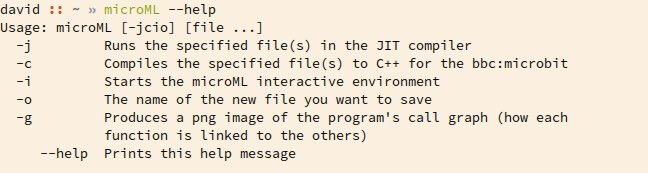
\includegraphics[width=\textwidth]{images/help.jpg}
    {\caption{MicroML command line help}}
\end{figure}

\begin{itemize}
    \item Download the repository from Git \url{https://github.com/kellino/microML}
    \item Unzip the repository and cd into the directory.
    \item run installMicroML
\end{itemize}

Assuming the build has been successful, typing `microML --help' into the terminal shows the various options. See Figure~\ref{fig:help}.


